\documentclass[]{IEEEtran}

\title{Modellazione e Sintesi di un Moltiplicatore Floating-point Single Precision}
\author{Enrico Sgarbanti - VR446095}

\usepackage{graphicx}
\usepackage[italian]{babel}

\begin{document}
\maketitle

\begin{abstract}
Il progetto ha 3 diversi obiettivi:
\begin{itemize}
\item Sviluppare in VHDL, Verilog e SystemC un componente che esegua due moltiplicazioni in virgola mobile a precisione singola
\item Sintetizzare i componenti scritti in VHDL e Verilog
\item Eseguire High-Level-Synthesis del moltiplicatore a precisione singola
\end{itemize}
\end{abstract}


\section{Introduzione}
Il sistema è composto da un modulo top-level chiamato ``double\textunderscore multiplier'' il quale esegue la moltiplicazione di due operandi dati in input nello stesso ciclo di clock in cui ready viene posto a 1, e i due opereandi passati al ciclo di clock successivo
\\

Nell'introduzione viene descritto in maniera astratta quello che poi viene dettagliato nel seguito del report. Una buona scaletta per l'introduzione pu\`o essere la seguente:
\begin{itemize}
\item Descrizione ad alto livello delle principali caratteristiche del sistema che si vuole modellare.
\item Descrizione delle motivazioni principali per l'utilizzo delle tecnologie descritte nel corso. Qual'\`e il problema che si vuole risolvere?
\item Descrizione dei passi utilizzati per arrivare all'implementazione finale. Descrivere la motivazione di ciascun passo. La descrizione dei passi dovrebbe formare la descrizione del flusso di lavoro svolto per completare l'assignment.
\item Rapidissima descrizione dei risultati principali.
\end{itemize}

L'introduzione non dovrebbe andare oltre la met\`a della seconda colonna (nel caso a due colonne), o la prima pagina (nel caso a colonna singola): bisogna cercare di essere concisi (e chiari). Alla fine, l'introduzione \`e solo ``chiacchiere'': deve semplicemente rendere chiari quali sono gli obiettivi del lavoro (\emph{e nel caso del corso, deve far capire a me che avete gli obiettivi chiari in testa}). Consiglio: l'introduzione (e spesso l'abstract) \`e l'ultima parte che viene completata.

\section{Background}

- descrivere cos'è un floating-point
- descrivere la moltiplicazione

Il background dovrebbe contenere una descrizione, abbastanza breve, dei concetti principali che vengono utilizzati nel lavoro. Ad esempio, pu\`o contenere una breve descrizione delle caratteristiche principali degli HDL , e delle sue estensioni. Una colonna dovrebbe bastare.

In questa sessione saranno citati anche lavori dello stato dell'arte. Ad esempio, si pu\`o usare~\cite{SystemC} per citare SystemC. \textbf{I riferimenti bibliografici vanno inseriti ogni volta in cui si va a citare qualcosa contenuto in un documento.}

Questa sessione non deve ripetere quanto detto a lezione, ma dare un overview dei concetti principali utilizzati durante lo svolgimento dell'elaborato.


\section{Metodologia applicata}
Per la realizzazione di questo progetto sono necessari 3 moduli:
\begin{itemize}
\item modulo del moliplicatore
\item modulo di alto livello che gestisce la moltiplicazione delle due coppie di operandi
\item modulo di testbench
\end{itemize}

\subsection{Modellazione delle EFSM}
Per la realizzazione del moltiplicatore sono necessari i segnali:
\begin{itemize}
\item ``rst'' (1 bit) per riportare il sistema allo stato iniziale 
\item ``ready'' (1 bit) per permettere al sistema di uscire dallo stato iniziale 
\item ``done'' (1 bit) per indicare che il valore attuale di ``res'' è il risultato della moltiplicazione
\item ``norm\textunderscore again'' (1 bit) per indicare se fare un'altra normalizzazione del numero intermedio
\item ``res\textunderscore type'' (2 bit)
\end{itemize} ` e un segnale a 1 bit `` 

 Esso necessita di 14 stati:
\begin{itemize}
\item START: Esso e lo stato iniziale del moltiplicatore e ha il compito di inizializzare i 
\end{itemize}

In questa sezione viene descritto tutto il procedimento, ed \`e dunque la sezione pi\`u importante del report. Va descritto passo passo quello che avete fatto, facendo capire ``esattamente'' cosa \`e stato fatto.

Questa sezione pu\`o essere divisa in sottosezioni. Le informazioni riportate nella lista seguente dovrebbero essere identificabili nel testo del report (\textbf{anche in ordine diverso}):
\begin{itemize}
\item Definizione dell-architettura del programma
\item Descrizione del componente di HW digitale.
\item Processo di ``sintesi'' verso RTL. Definizione dei sottocomponenti del componente HW, e della sua struttura. Definizione dell'interfaccia RTL, definizione della Macchina a Stati Finiti Estesa (EFSM) del componente e dei sottocomponenti. Realizzazione del componente HW utilizzando i processi in diversi stili a livello RTL. \`E inoltre possibile discutere la scelta dei tipi di dato.
%\item Descrizione della realizzazione della parte rappresentante SW Embedded, e descritta in TLM.
%\item Descrizione della realizzazione della parte a tempo continuo. Spiegazione delle scelte progettuali fatte per gli stili di modellazione utilizzati.
\item Descrizione dei meccanismi di comunicazione tra le diverse parti del sistema.
\end{itemize}

\textbf{In questa sezione deve essere riportato (brevemente) anche l'organizzazione dell'implementazione consegnata assieme al report.}

\section{Risultati}

Qua vanno ``messi i numeri''. Questa sezione dovrebbe contenere i risultati della simulazione. La simulazione mostra che il sistema funziona correttamente? Come \`e stato provato? Che tipo di testbench sono stati utilizzati? Come \`e stato scomposto il sistema per verificarne la correttezza?

Per quanto riguarda le performance:
\begin{itemize}
\item cosa si pu\`o dire in merito alla latenza?
\item Qual è la frequenza massima del design? 
\item Qual è l'area occupata dal design? 
\end{itemize}

Questa sezione pu\`o contenere anche riflessioni personali sui risultati ottenuti. Importante: tutte le affermazioni devono essere supportate da numeri\footnote{Richard Feynman on Scientific Method (1964) -\\ https://www.youtube.com/watch?v=OL6-x0modwY}.

\section{Conclusioni}
Le conclusioni dovrebbero riassumere in poche righe  tutto ci\`o che \`e stato fatto. Un paio di righe descrivono i risultati osservati, in modo da introdurre poi la conclusione ``vera e propria''. Nel caso del corso, la ``lezione da portare a casa'' sar\`a quello che si \`e imparato svolgendo l'elaborato.


\bibliographystyle{IEEEtran}
\bibliography{biblio}

\appendix
Se non avete abbastanza spazio, potete inserire le figure delle EFSM in una  pagina extra, appendice. Un esempio di come potete fare solo le Figure~\ref{fig:grande}, \ref{fig:piccola1}, \ref{fig:piccola2}.


\begin{figure*}[bt]
\centering
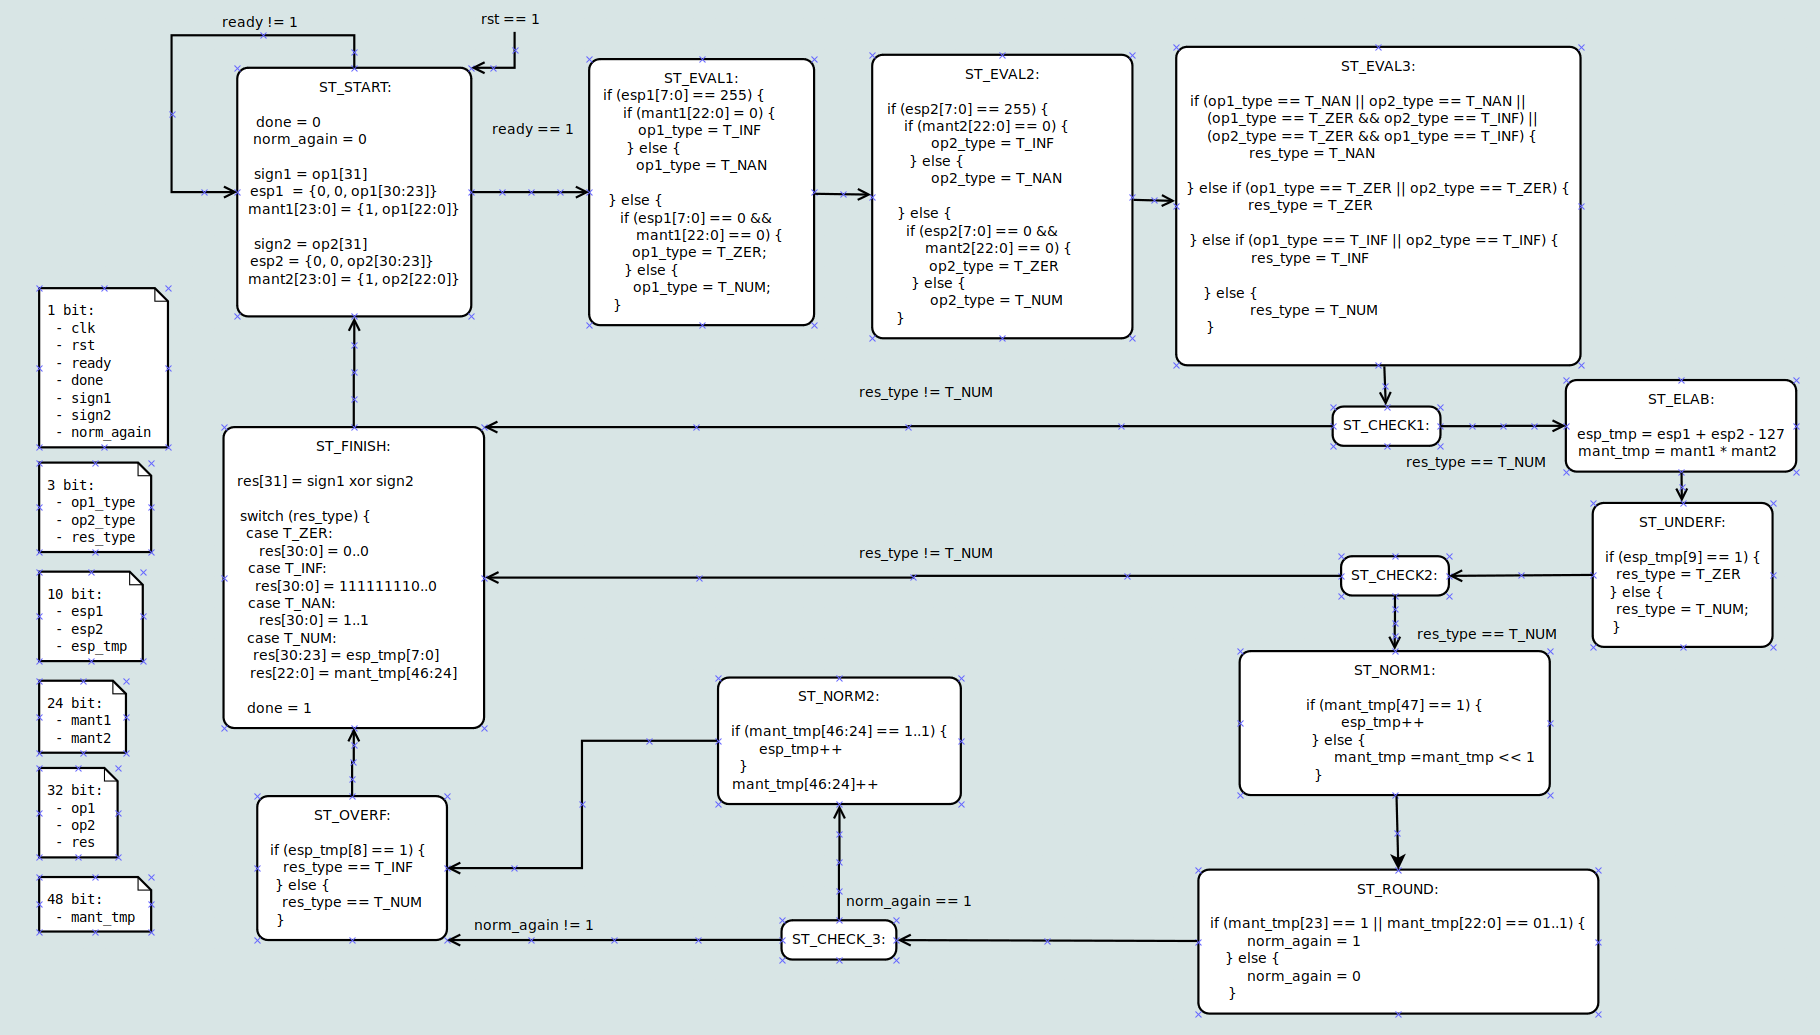
\includegraphics[width=\textwidth]{figures/EFSM-multiplier}
\caption{Figura in formato grande.}
\label{fig:grande}
\end{figure*}

\begin{figure}[bt]
	\centering
	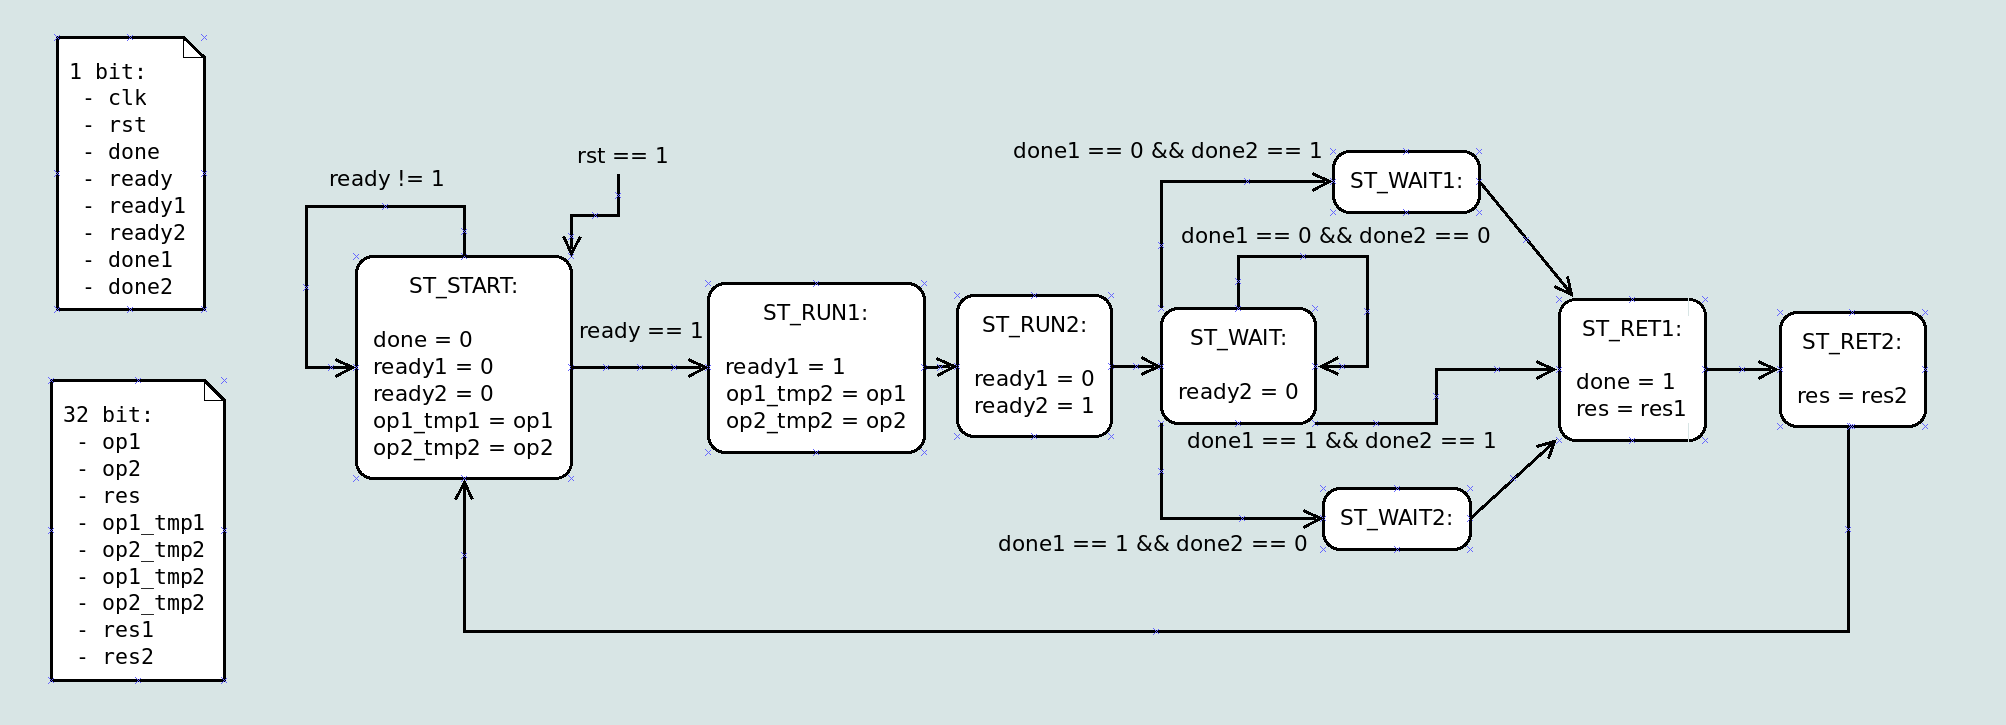
\includegraphics[width=\columnwidth]{figures/EFSM-top_level}
	\caption{Figura in formato piccolo, 1.}
	\label{fig:piccola1}
\end{figure}

\begin{figure}[bt]
	\centering
	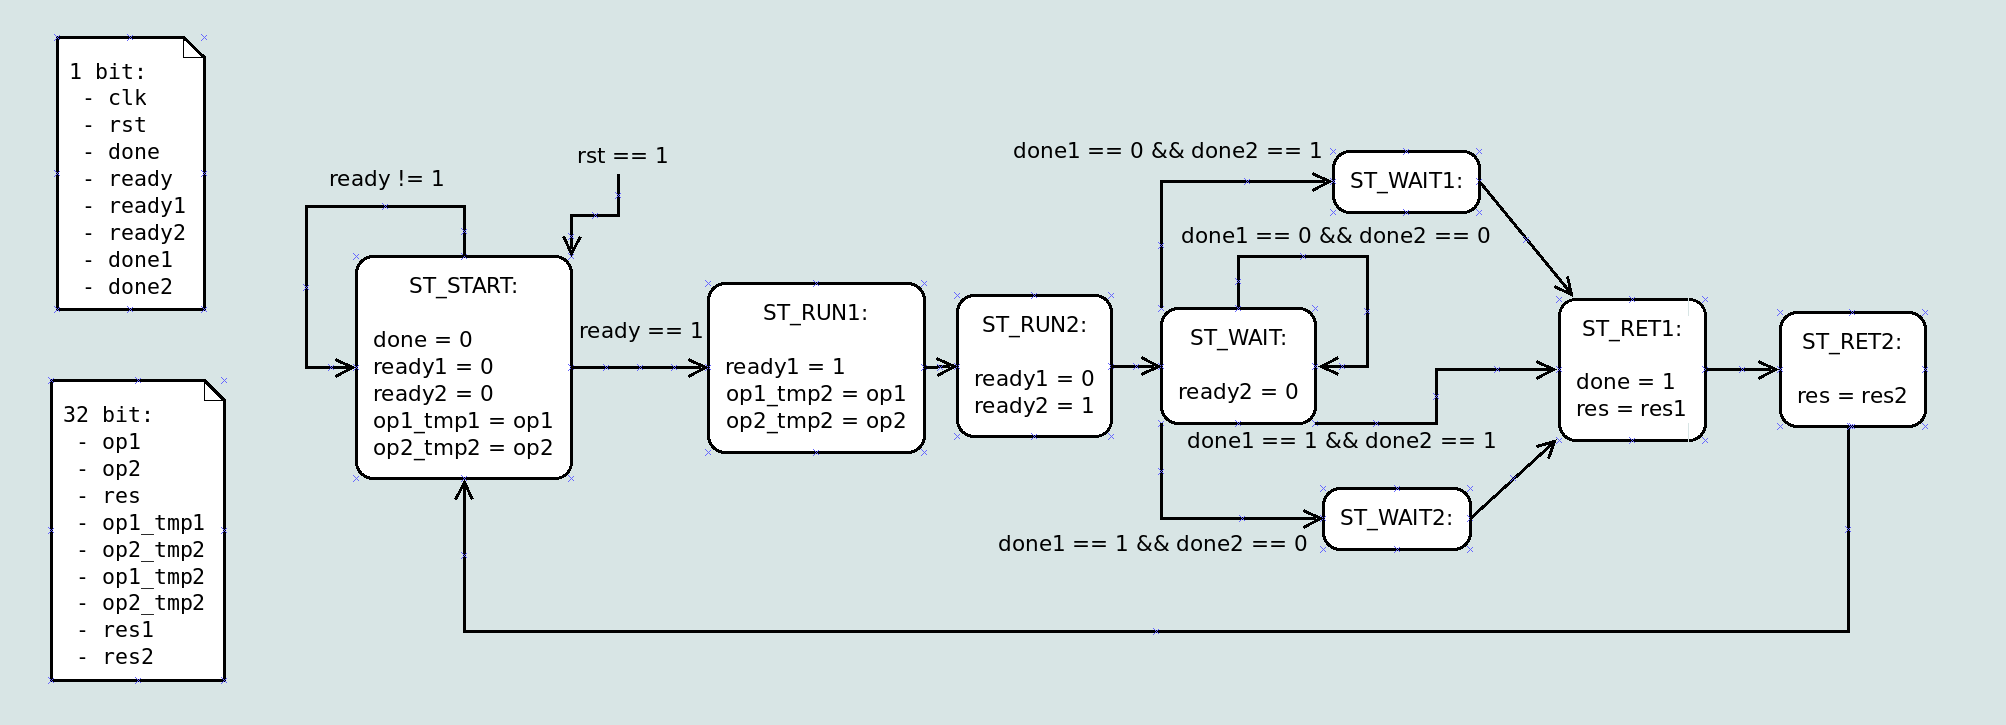
\includegraphics[width=\columnwidth]{figures/EFSM-top_level}
	\caption{Figura in formato piccolo, 2.}
	\label{fig:piccola2}
\end{figure}

\end{document}